\documentclass[11pt]{article}
\usepackage{amssymb}
\usepackage{tikz}
\usepackage{fancyhdr}
\usepackage{extramarks}
\usepackage{pgfplots}
\usetikzlibrary{automata,positioning}
\usetikzlibrary{shapes.geometric, arrows}


\setlength{\topmargin}{-1.5in}
\setlength{\textheight}{9.5in}
\setlength{\oddsidemargin}{.125in}
\setlength{\textwidth}{6.25in}

\tikzstyle{startstop} = [rectangle, rounded corners, minimum width=3cm, minimum height=1cm,text centered, text width=3cm, draw=black, fill=red!30]
\tikzstyle{basicblock} = [rectangle, minimum width=3cm, minimum height=1cm,text centered, text width=3cm, draw=black, fill=blue!30]

\tikzstyle{io} = [trapezium, trapezium left angle=70, trapezium right angle=110, minimum width=3cm, minimum height=1cm, text centered, text width=2cm,draw=black, fill=blue!30]
\tikzstyle{process} = [rectangle, minimum width=3cm, minimum height=1cm, text centered, text width=2cm,draw=black, fill=orange!30]
\tikzstyle{decision} = [diamond, minimum width=3cm, minimum height=1cm, text centered, text width=2cm, draw=black, fill=green!30]



\tikzstyle{arrow} = [thick,->,>=stealth]
\begin{document}
	\title{
		\textbf{Car Logic Architecture}
	}
	\date{}
	\maketitle

	\begin{tikzpicture}[node distance=2.5cm]


% Launch script

	\node (launchd) [startstop, xshift=1cm] {Launchd};


% Simulations

	\node (sumo)[basicblock, below of=launchd, xshift=-3cm] {Sumo};

	\node(omnet)[basicblock, below of=launchd, xshift=3cm]{Omnet};


% Car stack

	\node (hardwareSim)[basicblock, below of=sumo] {Hardware simulation};

	\node (agents) [basicblock, below of=hardwareSim] {Agents};


% Network stack

	\node(omnetPY)[basicblock, below of=omnet]{Omnet interface};

	\node(meshNet)[io, below of=omnetPY]{Mesh Network};


% API

	\node (carLogicAPI)[io, below of=agents, xshift=3cm]{Car Logic API};




% Launchd statement arrows

	\draw [arrow] (launchd) -| node[ anchor=east, yshift=-1cm]{Open Sumo} (sumo);
	\draw [arrow] (launchd) -| node [anchor=west, yshift=-1cm]{Open Omnet}(omnet);



% Omnet - Sumo connection
	\draw [arrow] (omnet.170)--(sumo.10);
	\draw [arrow] (sumo.350)--(omnet.190);


% Network Stack
	\draw [arrow] (omnet.250) -- (omnetPY.110);
	\draw [arrow] (omnetPY.70) -- (omnet.290);

	\draw [arrow] (omnetPY.250) -- (meshNet.110);
	\draw [arrow] (meshNet.70) -- (omnetPY.290);


% Hardware Stack
	\draw [arrow] (omnetPY.190) -- (hardwareSim.350);
	\draw [arrow] (hardwareSim.10) -- (omnetPY.170);

	\draw [arrow] (hardwareSim.250) -- (agents.110);
	\draw [arrow] (agents.70) -- (hardwareSim.290);


% Car logic API connects
	\draw [arrow] (meshNet.250) |- (carLogicAPI.10);
	\draw [arrow] (carLogicAPI.350) -| (meshNet.290);

	\draw [arrow] (agents.290) |- (carLogicAPI.170);
	\draw [arrow] (carLogicAPI.190) -| (agents.250);


	\end{tikzpicture}

	\begin{enumerate}
		\item Launchd: The first thing to run. This will be a python script
			that opens up the sumo simulation, opens omnet simulation, connects them
			with veins, and then launches the loop controller.
		\item Sumo: A sumo road simulation. See tutorials for more.
		\item Omnet: A omnet network simulation. See tutorials for more.
		\item Hardware simulation: This code will interpret the "World" view that
			sumo gives, and will return what is visible from any one car. Will emulate
			the Autonomous driver component of the final implementation, gives abstact
			information, not "raw". Also accepts abstract requests, such as "Switch lanes",
			just as the Autonomous Driver Would.
		\item Omnet interace: Abstract out the omnet specific commands
		\item Mesh network: Control connections and message handeling. Generally
			handles all of the mesh network specific work.
		\item Car Logic API: a standard set of methods that the agent can interact
			with to join and contribute to the swarm of cars on the road.
		\item Agents: A swappable module, each representing a different manufacturer
			implementation of the Car Logic API, showing that different designs can
			all work using the API. The agent will 1) request information from the
			hardware simulation 2) get any new messages from the car logic api 3) decide
			what it wants to do 4) broadcast any relevant information to other cars
			5) request specific manuvers from the hardware simulation.
	\end{enumerate}
\end{document}
